Fabrication of a chip has been an iterative process, where we have
simultaneously improved upon both the chip's design and our fabrication
techniques.
In this chapter I will present the progress that we have made in
learning how to build a chip trap, and how we plan to integrate a microwave
guide in future experiments. 

All the microfabrication techniques described below except for the
electroplating were undertaken at the London Centre for Nanotechnology (LCN). 

\section{Overview of the fabrication procedure}

% TODO I grabbed this Madou2002 citation from Treutlein, but I should ensure
% that it is legit
Our trap has been designed so that the size of the wires is small compared to
the size and height of the trapped cloud. As such trapping wires on the chip
are as small as \SI{3}{\micro\meter} in width. Such small features can be
produced using standard photolithography techniques~\cite{Madou2002}. However,
the maximum height of features produced in these procedures is usually of the
order \SI{100}{\nano\meter}.

% TODO Need to cite this $j$ number and probably revise this based on what we
% actually say in design chapter. I don't think I need this caluclation here
We must ensure that the wires are capable of carrying the currents that are
outlined in chapter~\ref{design}.  Other experiments with two-layer atom chips
have reported a current density of $j=\SI{6E10}{\ampere\per\meter\squared}$ in
the trapping wires. For our wires this would require a minimum height of $h
\sim I w/j = \SI{1}{\ampere} \times
\SI{10}{\micro\meter}/\SI{6E10}{\ampere\per\meter\squared} \sim
\SI{1}{\micro\meter}$  to carry our trapping currents.This is much higher than
can be achieved with photolithography techniques.

To achieve the required height, we have used through-mask
electroplating~\cite{Ruythooren_2000}. First a substate is coated with a thin
seed layer of gold, then photolithography is used to produce a thick (several
mircron high) mould. The mould covers regions where no further deposition is
required. The substrate can then be electroplated, with the seed layer acting
as the anode, allowing thick wires to be deposited into the mould.
After electroplating the seed layer can be etched away. This is a common
technique for constructing atom chips and is described in \inlinerefs{2011Ac,
Lev2003, KOUKHARENKO2004600}.

The fabrication process for our final chip begins with a four inch silicon
wafer, which we dice into individual \SI{20}{\milli\meter} by
\SI{20}{\milli\meter} dies. The remaining process can be briefly summarised:
\cm{Is there a better way to link this list to the following sections?}
\begin{enumerate}
  \item Dice silicon wafer into \SI{20}{\milli\meter} by \SI{20}{\milli\meter}
    dies.
  \item Evaporate adhesion layer of chromium.
  \item Evaporate seed layer of gold.
  \item Spin coat a thick (\SI{6}{\micro\meter}) layer of photoresist.
  \item Expose photoresist to pattern the die.
  \item Develop photoresist to create photoresist mould.
  \item Electroplate the chip, such that wires are formed in the mould to the
    desired height.
  \item Remove the photoresist mould.
  \item Chemically etch the gold seed layer.
  \item Chemically etch the chromium adhesion layer so as to remove the seed.
    layer and electrically isolate the wires.
\end{enumerate}
This process is illustrated in \myfigref{fab:fig:process}

\begin{figure}[p]
\vspace{0.8cm}
\centering
  \begin{overpic}[width=\textwidth]{figs/fab/cartoon/wholeprocess.pdf}
    \put(04, 73){(1)}
    \put(28, 73){(2)}
    \put(52, 73){(3)}
    \put(76, 73){(4)}
    \put(04, 60){(5)}
    \put(28, 60){(6)}
    \put(52, 60){(7)}
    \put(76, 60){(8)}
    \put(04, 9){(9)}
    \put(28, 9){(10)}
    \put(52, 9){(11)}
    \put(76, 9){(12)}
    \put(3.5,24.5){$h$}
    \put(25.5,16.75){$x$}
  \end{overpic}
  \caption[Illustration of the fabrication process]{
Illustration of the fabrication process. We begin with a bare silicon die
(black) which has already been cut to the desired size, and is shown here in
profile. We evaporate a chromium adhesion layer (2, grey) followed by the gold
seed layer (3, gold).  A thick ($\sim6\si{\micro\meter}$) layer of photoresist
(purple) is spin coated (4).

Steps \numrange{5}{8}, highlighted in the grey box, include a more detailed
overview of through-mask electroplating, with a top-down view (top row), profile
view (second row) and profilometer scan (bottom row). The dashed line denotes
the cut for the profile view and profilometer scan. In (5) a region of
photoresist (blue) is exposed to the UV light by raster scanning (black lines) of
the direct writer. The die is then developed (6) to create a photoresist mould,
which can be electroplated to build tall wires (7). Removing the mould (8)
leaves only the tall wires, and the initial metal layers.

The gold and then chromium layers are etched (9 and 10) to isolate the
features. Planned further fabrication steps are shown in the box. We
intend to spin coat with polyimide (11, pink), allowing fabrication of features
such as microwave guides on a second layer above the trapping wires (12).
  }
  \label{fab:fig:process}
\end{figure}

As discussed in chapter~\ref{intro}, a future aim of the molecule chip project is to
integrate microwave guides on the chip. These guides must allow good overlap of
the microwave fields and the molecule trapping region. Our design achieves this
by positioning the microwave guides on a second layer, directly above the
trapping wires. We have not yet attempted the following stages of
fabrication, but we anticipate that they will be:
\begin{enumerate}[resume]
    \item Spin coat chip with an insulating layer of polyimide.
    \item Perform standard photolithography to lay down microwave guides on the
      chip.
\end{enumerate}
These steps are discussed further in section~\ref{fab:planned}.

In the rest of this chapter I will describe the above process in detail,
including the various pitfalls that we found as we itterated towards a complete
\cm{trapping chip}.

\section{Metal evaporation of seed layer}

Before any fabrication, the die must be cleaned and dehydrated to ensure that
there will be good adhesion to the substrate. A solvent clean with acetone and
isopropyl alchol will remove any organic compounds \cm{check this}. The die is
then rinsed with deionised water and dehydrated in an oxygen plasma for ten
minutes.
The die is then ready for metalization, which here is done by metal
evaporation. To further improve adhesion between the gold and silicon, a thin
($<10\si{\micro\meter}$) intermediary chrome layer is deposited first, followed
by \SI{50}{\micro\meter} of gold.

We performed evaporation using an Edwards A306 bell jar evaporator. Typically
we \cm{metalize} four dies at a time. They are loaded into the belljar, along
with gold and chrome, using a boat and rod respectively.  we deposit gold onto
four dies at a time. The dies are positioned with the polished side facing down
towards the metal. This arrangement is shown in \myfigref{fab:fig:belljar}.

\begin{figure}
  \centering
  \begin{subfigure}[b]{0.22\textwidth}
    \centering
    \begin{overpic}[width=\textwidth]{figs/fab/cartoon/evap.pdf}
      \put(48,6){$I$}
    \end{overpic}
    \caption{}
  \end{subfigure}
  \hspace{2cm}
  \begin{subfigure}[b]{0.22\textwidth}
    \centering
    \includegraphics[width=\textwidth]{figs/fab/belljar.png}
    \caption{}
  \end{subfigure}
  \caption{
    Subfigure (a) schematically shows evaporation of gold (yellow) onto a
    silicon (black) die with chromium (grey) adhesion layer. The shutter
    (dashed line) can block the evaporating gold from being deposited when
    the target height is reached. The Edwards belljar evaporator is shown in
    (b), with the belljar removed and a wafer mounted for deposition.
  }
  \label{fab:fig:belljar}
\end{figure}

The belljar is pumped down to pressures below $10^{-6}\si{\milli\bar}$ over a
few hours. The metal for deposition can be selected from a carousel, and heated
by electric current inducing evaporation.  A shutter is used to block
deposition onto the substrate until the desired current has been reached. It is
then opened to begin deposition.
The Edwards bell jar evaporator incorporates a FTM7 deposition monitor, which
reports the rate of deposition and automatically shuts off deposition once the
desired thickness has been reached by closing the shutter. \cm{What
determines/ limits the deposition rates? What happens when we have too much
current?}

The deposition rate of gold is typically \SI{0.2}{\nano\meter\per\second}.
%
\cm{Find a way to cite LCN for this and maybe some other factoids.}
%
As discussed above a thickness of \SI{5}{\micro\meter} is desirable for the
chip's trapping wires. Achieving this with evaporation would take over an hour,
and it would not be possible to load the evaporator with enough gold to last
this long. This is why we must use electroplating to achieve the desired
thickness.

\section{Spin coating of photoresist}
\label{fab:spin}

Spin coating is a procedure for distributing a uniform layer of liquid such as
photoresist  across a substrate~\cite{Cohen2011}. It is typically followed by
baking to solidify the layer. We use spin coating to apply Dupont SPR220-7
\cite{} photoresist, which will form the mould for the wires.

The die is mounted in a spin coater, and approximately \SI{1}{\milli\meter} of
SPR220-7 is appled. The die undergoes a \cm{\SI{2}{\second} ramp to
\SI{500}{\rpm} where it is held before a second ramp to \SI{4000}{\rpm} and
held for \SI{30}{\second}.} This results in a nominal \SI{6}{\micro\meter} high
coating of photoresist. SPR220-7 requires a post-application bake, first at
\SI{90}{\celsius} for two minutes, then immediately afterwards at
\SI{120}{\celsius}.

Spin coating the photoresist results in a bead at the edge of the die. This
thick region of photoresist may not receive sufficient exposure to fully
develop later. This can cause defects in features near the edge. It is
possible to remove the bead by inserting an intial exposure and development
step before the lithography discussed in the next section. However, since the
only features that are covered by the bead are the robust wire bond pads, this
is deemed unnecessary for our purposes. \cm{Defects due to the presence of a
bead can be seen in \myfigref{}.} Using too much photoresist during coating can
produce an unduly thick bead, which can further interfere with photolithography
steps.

\section{Lithography of the wire mould}

The common and, perhaps, traditional way to perform photolithography is to use
a mercury lamp and a chrome-on-glass mask to cast light onto the
substrate, with the mask casting a shadow so as to illuminate only the desired
region~\cite{Madou2002}. This was the method that we began using at the start of the
project, however we found that it was easier to achieve reliable results by
using the the Heidlberg DWL 66, a direct writer~\cite{}. 

Instead of using a mask to cast a shadow, the direct writer uses a tightly
focused ultraviolet laser, whose beam is raster scanned across the surface. The
beam is then switched on and off so as to produce the pattern that is required.
This process is depicted for a in \myfigref{fab:fig:methods}. The Heidelberg
DWL 66 is capable of producing features down to \SI{300}{\nano\meter} in size.

Since designs can be directly uploaded to the direct writer, there is no need
to wait for a third party to construct a mask.  Hence the direct writer allows
rapid prototyping. It also has the benefit of making alignment easier, since
this can be performed automatically by the computer, and any issues with
mask-die contact are avoided entirely. 

The SPR220-7 is a positive photoresist, meaning that areas exposed to the light
are those which will be removed on developing. It has an exposure energy of
\SI{140}{\milli\joule\per\square\centi\meter} is required, which is
administered over three passes. The laser power is calibrated to achieve the
correct exposure of the laser, operating at \SI{70}{\milli\watt}. The
whole scan for one die takes around twenty minutes. This process is illustrated
in \mysubfigref{fab:fig:process}{5}.

Following exposure a rehydration step is required. The die is left at ambient
temperature overnight before it is developed in Microposit MF-319 until it runs
clear, and then for \SI{30}{\second} extra (usually about two minutes total).
This produces the die with mould as depicted in
\mysubfigref{fab:fig:process}{6}.

\subsection{Troubleshooting}

A common problem that we faced early in development was underexposing the
photoresist. This meant that some features were entirely missing from the mould,
and others were incomplete, with photoresist remaining at the bottom of the
mould after developing. This blocks the current during electroplating, and
prevents the formation of wires. This can be seen with the microscope, and is
confirmed when electroplating dies where the underdevelopment is present.

\begin{figure}[h]
\end{figure}
\begin{figure}
  \centering
  \begin{subfigure}[b]{0.45\textwidth}
    \centering
  \begin{overpic}[width=\textwidth]{figs/fab/mould/wafer1_mould_scale.png}
    \put(16,18){\SI{50}{\micro\meter}}
  \end{overpic}
    \caption{}
  \end{subfigure}
  \hspace{1cm}
  \begin{subfigure}[b]{0.45\textwidth}
    \centering
  \begin{overpic}[width=\textwidth]{figs/fab/mould/wafer2_mould_scale.png}
    \put(15,18){\SI{50}{\micro\meter}}
  \end{overpic}
    \caption{}
  \end{subfigure}
  rcaption{
    Photoresist moulds for \ph{design one} dies. In (a) we see the effects of
    underexposure, features below $\sim20\si{\micro\meter}$ are completely
    absent. The \SI{20}{\micro\meter} wire is present but has not been
    completely developed. Subfigure (b) shows a well-exposed die of the same
    design, with sharp features and clear trenches in which the wires can be
    plated.
  }
  \label{fab:fig:moulds}
\end{figure}

Even after proper exposure it is possible that the photoresist can be
underdeveloped. This yields similar problems to underexposure, but can be
easily resolved by returning the die to the developer. 


\section{Electroplating the tall wires}

Now the chip is returned to the Blacket Laboratory for electroplating.
Electroplating does not take place in cleanroom conditions, but it is important
that the dies are treated with great care during transport, and kept sealed
until electroplating can begin. We found that the dies were surprisingly
robust, and were able to be kept for several weeks between exposure and
electroplating.

In electroplating, a conductive target (here, the die) is connected to an
electric circuit as an anode and placed into an electrolytic solution along
with a cathode. Current passed through the solution causes ions in the solution
to be deposited onto the target. This is illustrated in
\mysubfigref{fab:fig:etch}{a}, and the results of the process are shown
schematically in \mysubfigref{fab:fig:process}{\cm{9 and 10}}. An overview of
electroplating can be found in \inlineref{Schlesinger2011}.
%
\cm{This ref again, check it is ok!}

Here we use the through-mask electroplating method to deposit thick gold wires
into the regions that are not covered by the photoresist mould, as shown in
\myfigref{fab:fig:eplate}. This method allows us to produce wires up to the
thickness of the photoresist height. Above this the wires will begin to
``mushroom,'' spreading out across the top of the photoresist and losing their
shape. As per the discussion in \cm{ref chapter}, we require a minimum wire
height of \cm{\SI{5}{\micro\meter}}. We will see below that we have been able
to reliably produce wires up to a height of \SI{6}{\micro\meter}.

\begin{figure}
\vspace{0.8cm}
\centering
  \begin{subfigure}[b]{0.22\textwidth}
    \centering
  \begin{overpic}[width=\textwidth]{figs/fab/cartoon/eplate.pdf}
    \put(28.7,91.2){$I$}
  \end{overpic}
    \caption{}
  \end{subfigure}
  \hspace{2cm}
  \begin{subfigure}[b]{0.22\textwidth}
    \centering
    \includegraphics[width=\textwidth]{figs/fab/eplate.png}
    \caption{}
  \end{subfigure}
  \caption{
    The elecroplating scheme is shown schematically in (a). A die is submerged in a gold electrolyte
    (light blue) along with an electrode (grey mesh). These are connected to a
    current supply to enable current flow and deposition of gold ions (yellow
    circle)  is depicted. The solution is held at \SI{60}{\celsius} and
    agitated by a stirrer and bubbler. A photograph of our apparatus is shown
    in (b). The beaker containing the electrolyte is submerged in a water bath
    and aggitated with a stirrer and bubbler.
  }
  \label{fab:fig:eplate}
\end{figure}

The height $h$ achieved in a deposition of duration $t$ is given by the Faraday
equation~\cite{Ruythooren_2000}
%
\begin{equation}
  h = \left(\frac{\alpha I M}{nFA\rho}\right)t
  \label{fab:eqn:faraday}
\end{equation}
%
where $I$ is the current, $F=\SI{96.5}{\kilo\ampere\second\per\mole}$ is the
Faraday constant, and other parameters with values specific to our gold
deposition are: $\alpha\sim0.9$, the current efficiency; $M =
\SI{197}{\gram\per\mole}$ the molar mass;
$\rho=\SI{19.32}{\gram\per\centi\meter\cubed}$, the density of the deposited
metal; $n=1$, the charge on the deposited ions in units of electron charge; and
$A\sim\SI{1}{\centi\meter\squared}$ is the area for plating.

We therefore have a relationship between the current, the target height and the
time,
%
\begin{equation}
  h \approx \left(
  \SI[per-mode=fraction]{1e-10}{\meter\cubed\per\ampere\per\second} \right)
  \times\frac{It}{A}.
\end{equation}
%
\cm{Ensure I am not word stealing here...}
For our electrolytic solution, we have used Metakem Goldbath-SF.
Metakem Goldbath-SF is chosen because it produces very pure (99.99\%) deposits,
and will not react with our photoresist. The effectiveness of this product has
been demonstrated for a similar design in \inlineref{Treutlein2008}.
%
\cm{Should cite metakem}

Goldbath-SF is suitable for use with current densities in the range
\SIrange{1}{15}{\milli\ampere\per\centi\meter\squared}. Final chip design has a
plating surface area of $S\approx85\si{\milli\meter\squared}$. There is also an
additional contribution to surface area from the clip with which we hold the
die in place during plating. We therefore do not know the plating area
exactly, but we ensure that the entire clip in the solution every time to
ensure the results are reproducable. We can also estimate the minimum plating
time for wire heights of \SI{3}{\micro\meter}, which we expect to be
\cm{TODO}.

% Can we figure out the chip area from the offset of different plating times?

Our apparatus for the electroplating step is shown in
\mysubfigref{fab:fig:eplate}. The electrolytic solution is placed in a
beaker, which itself is placed in a water bath held at \SI{60}{\celsius}. The
bath is heated using a hotplate with magnetic stirrer. Some time is allowed for
thermalisation, during which it is imporant that the goldbath is covered to
prevent loss by evaporation.

When the goldbath has reached \SI{60}{\celsius} the target chip and the cathode
are submerged. The chip is held in position by a stiff insulated wire, which
also carries current to the seed layer. A multimeter can be used to ensure that
there is good electrical contact from the wire to the holder. The wire is
insulated, and we use the smallest clip possible so as to minimise gold plating
to the chip.  The cathode is a grid of platinised titanium which has been cut
to the size of our beaker.  This was also purchased from Metakem.

% Change this to show that electroplating without the aggitation didn't work
% The whole of the next three paragraphs needs to be turned into more of the
% narative of how we learned to electroplate. Including profiling results

A bubbler is placed to agitate the solution near to the chip surface. This in
combination with gentle stirring ensures good circulation of the solution and
hence prevents localised depletion of the ions near to the chip
surface~\cite{Schlesinger2011} \cm{also cite conversation with S Etienne?}.

After electroplating, dies are rinsed with deionised water, and the photoresist
is removed overnight with Dupont 1165 photoresist remover, as illustrated
in \mysubfigref{fab:fig:process}{8}. Dies are then
dried and stored for transport to the LCN cleanroom for the inspection and
final fabrication steps.


\subsection{Inspecting the wires}
\label{fab:inspwire}

After plating it is useful to inspect the dies uner a microscope. This can
confirm that the wires have been \cm{created} successfully, and that the there
is continuity along them, but it cannot tell us the height that was achieved
during plating. To measure the plating height we use a a stylus profilometer,
in this case the Bruker DektakXT.

A stylus profilometer operates by positioning a gold stylus onto the surface of
the die and dragging it in one direction. As the stylus comes into contact with
features its height will change, allowing a profile of the surface to be
measured. Profiling of a surface is illustrated in \myfigref{fab:fig:process}
and is also useful for examining the features after plating.

We determined experimentally that electroplating at $\SI{15}{\milli\ampere}$
for duration $\SI{400}{\second}$ reliably produced wires of height
\SI{5}{\micro\meter} above the seed layer. A typical example is shown in
\myfigref{fab:fig:chipprofile}, where we also show a profile of the photoresist
mould used to fabricate these wires.

\begin{figure}[h]
  \centering
  \begin{subfigure}[b]{0.3\textwidth}
    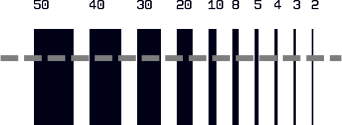
\includegraphics[width=\textwidth]{figs/fab/wiremouldprofile/lines.pdf}
    \vspace{1cm}
    \caption{}
  \end{subfigure}
  \hspace{1cm}
  \begin{subfigure}[b]{0.55\textwidth}
  \begin{tikzpicture}
    \begin{axis}[
        enlargelimits=true,
        xlabel=Scan distance (\si{\micro\meter}),
        ylabel=Height (\si{\micro\meter}),
        legend pos=outer north east,
        width=0.9\textwidth,
        height = 0.45\textwidth
    ]
    \addplot [
      color=purple,
      no marks,
      style=very thick
      ]
    table
    {figs/fab/wiremouldprofile/mould.dat};
    \addlegendentry{Mould}
    \addplot [
      color=gold,
      no marks,
      style=very thick
      ]
    table
    {figs/fab/wiremouldprofile/wire.dat};
    \addlegendentry{Wires}
    \end{axis}
  \end{tikzpicture}
    \caption{}
  \end{subfigure}
  \caption{Stylus profiling of the characterisation features. In (a) the lines
  feature of the chip is shown \ph{(c.f. earlier chapter)}, with the grey
  dashed line denoting the profile. Typical profiles are which is shown in (b),
  for both the photoresist mould and the plated wires. Stylus size limits the
  size of the trenches that can be fully profiled, and can make both trenches
  and hills appear narrower and wider respectively.
  }
  \label{fab:fig:chipprofile}
\end{figure}

Note that when examining the trenches of the mould with the profilometer, we
must account fo the finite size of the stylus.
The profilometer available at LCN is fitted with a gold stylus of radius
\SI{5}{\micro\meter}. This limits the resolution of the profile, hence why the
trenches in \myfigref{fab:fig:chipprofile} become distorted at and below
\SI{10}{\micro\meter}. This also means that the wires can appear to be slighly
wider, and the trenches slightly narrower, accounting for the overlap in the
figure.

\subsection{Troubleshooting}

Electroplating the dies was by far the most challenging stage of the
fabrication process.  It is therefore worth noting some of the complications
that we experienced and how they were overcome. 

% See OneNote 27 Nov 2019
Our first attempt at electroplating was with the photoresist mould shown in
\myfigref{fab:fig:moulds}, meaning that the full wires could not have been
formed. These were nonetheless sutiable targets for practice. We manually
agitated the electroplating solution during plating and were succesful in
laying down the larger features such as the wire bond pads, but sub
$\sim100\si{\micro\meter}$ features were not fabricated after removing the
photoresist mould. This can be clearly seen when inspecting the region around
the wire bond pads, as seen in \mysubfigref{fab:fig:aggandcorr}{a}.

We attempted to improve the adhesion with manual aggitation, and using a
bubbler, but eventually found that we achieved the best results with a
combination of gentle stirring and bubbling of the goldbath. This allowed us to
fabricate features up to around the \ph{limit imposed by our poor mould, as
described above}. However we found that our attempts to remove the photoresist
with acetone were ineffective, and resulted in the debris visible in
\mysubfigref{fab:fig:aggandcorr}{b}. It was resolved that this was unsuitable
and \ph{microposit 1165 remover} must be used instead.

For later attempts at electroplating we used a mould that had been exposed
correctly, shown in \ph{figure}. Combined with proper aggitation of the
solution and liftoff allowed fabrication of features to the
$1\si{\micro\meter}$ scale, as can be seen in
\mysubfigref{fab:fig:aggandcorr}{c} and (d). We can also see in these figures
that the smallest wires (\SI{10}{\micro\meter} and \SI{3}{\micro\meter}) have
been broken off from the surface of the die. This was due to sonicating the
chip during photoresist removal. 


% TODO Add a scale to these figs.
\begin{figure}
  \centering
  \begin{subfigure}[b]{0.45\textwidth}
    \includegraphics[width=\textwidth]{figs/fab/eplatetroubleshoot/aggandcorr/manualagg_flipped.png}
    \caption{}
  \end{subfigure}
  \hspace{1cm}
  \begin{subfigure}[b]{0.45\textwidth}
    \centering
    \includegraphics[width=\textwidth]{figs/fab/eplatetroubleshoot/aggandcorr/corrosion_flipped.png}
    \caption{}
  \end{subfigure}

  \begin{subfigure}[b]{0.45\textwidth}
    \centering
    \includegraphics[width=\textwidth]{figs/fab/eplatetroubleshoot/aggandcorr/goodpads.png}
    \caption{}
  \end{subfigure}
  \hspace{1cm}
  \begin{subfigure}[b]{0.45\textwidth}
    \centering
  \begin{overpic}[width=\textwidth]{figs/fab/eplatetroubleshoot/aggandcorr/goodcentre_scale.png}
    \put(69,18){\SI{50}{\micro\meter}}
  \end{overpic}
    \caption{}
  \end{subfigure}
  \caption{
    The effects of insufficient aggitation (a) and removal of the photoresist
    with solvents (b) can be compared to later results, where the solution is
    well aggitated during electroplating (c) and the photoresist is removed
    with \ph{1165 remover}. However the smallest wires were damaged by
    sonicating. The dies shown in (a) and (b) are different dies
    from the same batch. Subfigures (c) and (d) both show the same die, which
    was produced after the cause of both problems was identified. All three
    dies here have been electroplated at \SI{10}{\milli\ampere} for
    \SI{200}{\milli\second}.
  }
  \label{fab:fig:aggandcorr}
\end{figure}

To protect the fragile features we no longer sonicate the die during removal,
and instead submerge the die in the remover overnight. This was done with
\ph{the new design}, and we were able to electroplate features with a
resolution of up to \SI{3}{\micro\meter}. See figure \ph{a figure showcasing a
good chip with nice height including profiles}.

Note how the larger wires in \ph{above fig. again} were not uniformly plated,
with some areas near the edge seemingly shadowed by the mould as shown in
\cm{fig. showing shadowing}. This phenomenom was also noted in
\inlineref{Treutlein2008}, where it is suggested that the only solution is to
change to new goldbath. Indeed doing this and following the same procedure
produced results without this shadowing effect, see \cm{figure without
shadowing}.
%
% Could note that this is likely due to aging, as we started to see the effect
% after coming back from covid.

Although the shadowing was successful, we noted that the height of the wires
was very different between the two solutions for the same plating time and
currents. Dies \cm{C, D and E?} were all plated for \cm{Time and current}, but
\cm{C?} was plated with older solution yielding shadowing and \cm{D and E} were
plated with new solution without shadowing. The wires in \cm{C?} are \cm{3?}
times higher than those of \cm{D and E?} suggesting that the plating efficency
$\alpha$ varies between solutions. Plating of \cm{F} for \cm{twice as long as D
and E} produced wires of \cm{twice the height}, suggesting that the process is
consistent with \myeqref{fab:eqn:faraday}. The results from this plating are
examined in \cm{need a figure for this!}

\section{Etching}

The seed layer electrically connects the trapping wires, which is
essential for electroplating, but they must be separated for operation. This is
achieved by etching the metal.

Any thin films or other debris left on the die can become stuck to the chip
during etching. \cite{} Hence it is essential to ensure that the die is very
well cleaned (having been exposed to a non-cleanroom environment for
electroplating). We found that a solvent clean on its own was insufficient,
and would leave some residue on the die after the etch that we could not
remove, shown in \myfigref{fab:fig:etchres}. This was resolved by also cleaning
for ten minutes in an oxygen plasma, suggesting that this debris may have been
caused by residual photoresist.

% TODO Need a scale on these figures
% TODO Should I highlight and say something about the deformity due to the bead
% too?
\begin{figure}
  \centering
  \begin{subfigure}[b]{0.45\textwidth}
    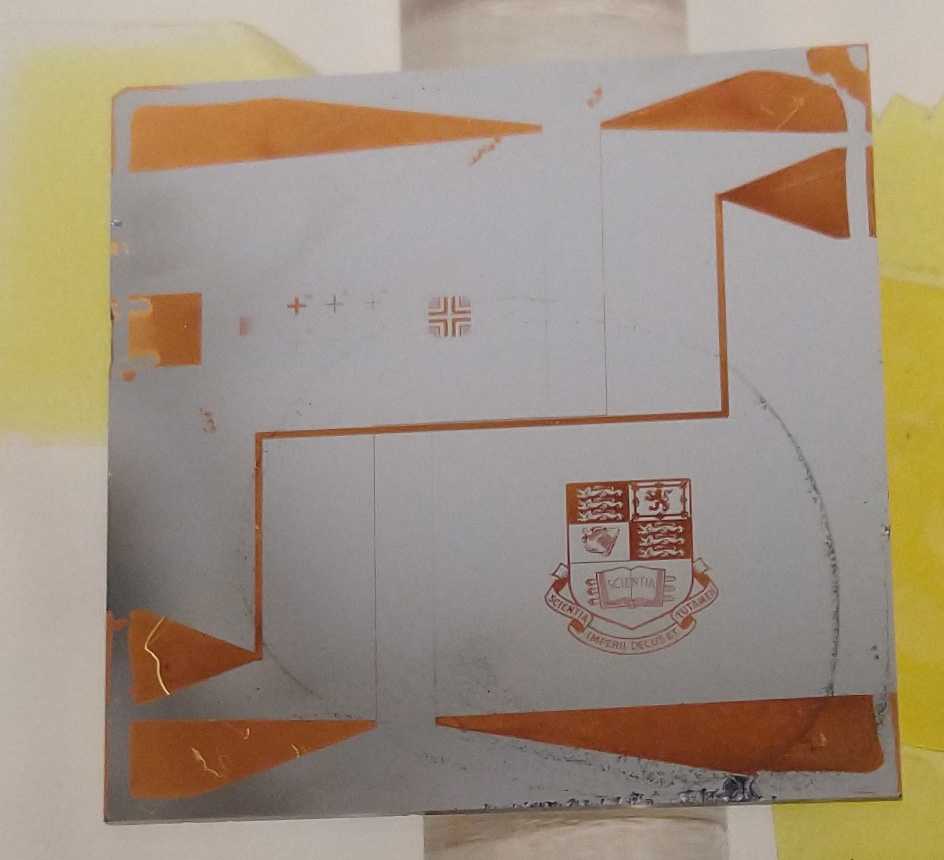
\includegraphics[width=\textwidth]{figs/fab/etch/etchdebris.jpg}
    \caption{}
  \end{subfigure}
  \hspace{1cm}
  \begin{subfigure}[b]{0.45\textwidth}
    \centering
    \includegraphics[width=\textwidth]{figs/fab/etch/etchdebris_scope.png}
    \caption{}
  \end{subfigure}
  \caption{Residue left on the die after etching. It was found that this can be
  avoided by cleaning with an oxygen plasma for ten minutes prior to etching.}
  \label{fab:fig:etchres}
\end{figure}

\cm{Need to figure out the actual name of the etchant, and check numbers}
%
After cleaning the gold etch is performed by placing the chip into a beaker of
Iodine etchant, which etches gold at a rate of \SI{5}{\nano\meter\per\second}.
This means that an etch of \SI{10}{\second} will remove the seed layer. After
this the chip is immediately transferred to a beaker of deionised water and
then rinsed. Since the seed layer thickness is significantly smaller than the
dimensions of the wire, the cross-sectional area will not be significantly
altered in this time.

\cm{Need to find out what the Cr etchant is called}
%
To complete the separation of the wires, the chromium layer must also be etched
in the same way. The process is the same as for the gold etch: the chip is
submerged in a beaker of the etchant and after the pre-determined exposure time
it is transferred to deionised water and then rinsed. This stage of the
fabrication is represented in \mysubfigref{fab:fig:etch}{d}. 

\section{Inspecting the finished die}

To ensure that the etches have been successful, stylus profiling is once again
performed, results are shown in \myfigref{fab:fig:endprofile}. We ensure that
the wires are of a sufficient height and width to achieve the required currents
as detailed in chapter~\ref{design}. Visual inspection under an optical
microscope is also useful to ensure that the silicon has been completely
exposed. A multimeter is used to confirm that there are no breaks in the wires.

\begin{figure}
\centering
  \includegraphics[width=0.8\textwidth]{figs/fab/wire_profile.pdf}
  \caption{A profile of trapping wires after etching, showing wires
  electroplated up to a height of approximately \SI{3}{\micro\meter}.
  \cm{Mike says I need to make a better version of this figure. This is on my
  todos, but I really want to do it for the new chip design.}
  }
  \label{fab:fig:endprofile}
\end{figure}

\section{Scaling fabrication}

In future design iterations it may be useful to scale the fabrication process
up by fabricating on the wafer scale rather than the scale of an individual
die. An entire wafer can be metallised, be spin coated and exposed to
produce the photoresist mask. Electroplating on the wafer scale may prove to be
more complicated than our comparatively small targets, but \cm{...}

\section{Planned fabrication of microwave layer}
\label{fab:planned}

In chapter~\ref{intro} 
we described how a molecule chip could allow strong coupling between \CaF{}
molecules and a microwave field, however for this to be possible there must be
good overlap between the microwave field and the trapped
molecules~\cite{Andre2006}.
%
\cm{better cite needed maybe?}

This overlap has previously been achieved for atoms in a magnetic
trap~\cite{Treutlein2008}. An insulating layer is spin-coated onto the trapping
wires so that a CPW \cm{In final version I need to check that first use of
abbreviation is explained.} can be fabricated by
photolithography. The trap centre can be positioned in the region where the
microwave field is strongest. This has potential to allow coherent control of
the molecules and potentially even sideband cooling into the motional ground
state~\cite{Andre2006}.
%
\cm{more discussion elsewhere?}

We will develop our fabrication procedure further so that we can produce such a
chip. The first stage will be to spin coat the insulating layer on top of an
etched chip, as shown in \mysubfigref{fab:fig:process}{11}. Again taking our
lead from \inlineref{Treutlein2008}, we will use polyimide. Polyimide is chosen
due to its low dielectric loss tangent ($\tan\delta_e = 0.016$) which will
minimise conductor losses in the waveguide~\cite{Collin2007, Simons2004}.
\footnote{Although a suitable dielectric is important to minimise conductor
losses in a CPW, this chip will operate at room temperature and so radiation
losses will dominate. This was discussed in detail in the early stage
assessment and will not be repeated here.}
%
\cm{This \emph{will} be repeated in the thesis so I can link this better.}

When spin coating the polyimide it is essential that we are able to produce a
flat surface onto which we can fabricate the microwave layer. We can do this by
applying multiple layers of polyimide on the spin coater, so that any bumps are
smoothed out. This is known as planarisation and is discussed further in
\inlineref{Treutlein2008}.

After the application of a planarised polyimide layer it will be possible to
fabricate microwave guides on the surface by lithography. The end result is
shown in \mysubfigref{fab:fig:process}{12}. We will undertake further work to
determine the required height of the CPW features and where they must be
positioned relative to the wires to achieve the strongest coupling.

\section{Connection to subchip}

% Check when I introduce initials here, could be in ch 1 or smth
To be used in the molecule experiment, the die must be mounted on the subchip
descirbed in \ph{an earlier chapter}.

\subsection{Gluing}

% Epoxy process and testing
First the die is glued into the mounting hole in the subchip with \ph{Epotex
resin}, an epoxy resin which is suitable for use in ultrahigh vacuum systems.
This is a two part resin, with parts A and B mixed in a five to one ratio by
weight. The two parts are measured out with a mass balance, and then a tiny
amount is applied to the subchip. Only enough resin is required that when the
die is pressed onto the surface there will be a miniscus between the surfaces
of the die and the subchip.

Placing the die into the mounting hole, the gluing is followed by pressing in a
vacuum bag. This presses the die into the resin and may help to prevent air
pockets in the resin, which could leak into the vacuum later.

Finally the entire assembly is baked at \SI{115}{\celsius} for an hour, then
left to cool.

\subsection{Wirebonding}

To form electrical connection between the subchip and the die, we wirebond
between the two.
